\section{Jump Land}

\begin{frame}
\frametitle{Jump Land}
\begin{block}{Problem: Jump Land}
There are $N \times N$ tiles. At the beginning, each tile is at height level $h_{ij}$ and each tile will move up by $v_{ij}$ units. How many tiles are adjacent to each other at the second with the most adjacent tiles?
\end{block}

\begin{center}
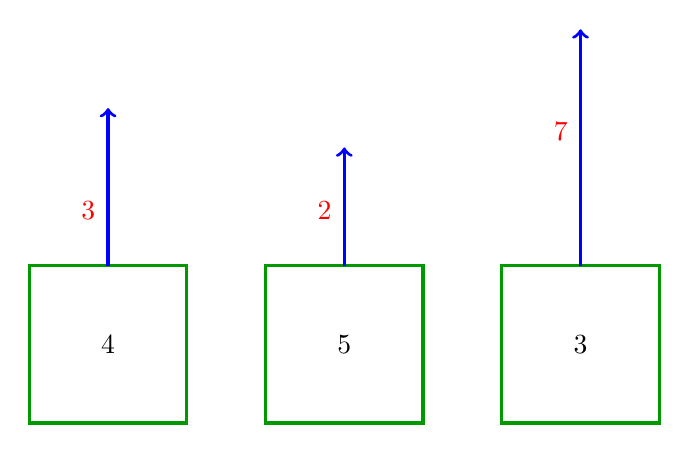
\begin{tikzpicture}
    \draw[green!60!black, very thick] (-3,0) rectangle (-1,2);
    \node at (-2,1) {4};
    
    \draw[green!60!black, very thick] (0,0) rectangle (2,2);
    \node at (1,1) {5};
    
    \draw[green!60!black, very thick] (3,0) rectangle (5,2);
    \node at (4,1) {3};
    
    \draw[blue, very thick, ->] (-2,2) -- (-2,4);
    \draw[blue, very thick, ->] (1,2) -- (1,3.5);
    \draw[blue, very thick, ->] (4,2) -- (4,5);
    
    \node[red] at (-2.25,2.7) {3};
    \node[red] at (0.75,2.7) {2};
    \node[red] at (3.75,3.7) {7};
\end{tikzpicture}
\end{center}

\end{frame}

\begin{frame}[fragile]
\frametitle{Jump Land}
We can store the time when two tiles are adjacent.

\begin{lstlisting}[language=C++, basicstyle=\small]
struct merge_t {
    int u, v;
    double t;
    merge_t(int _u, int _v, double _t):
        u(_u), v(_v), t(_t) {}
};
\end{lstlisting}

\end{frame}

\begin{frame}
\frametitle{Jump Land}
When will tile $a$ and tile $b$ adjacent?

There are $3$ cases:

\begin{enumerate}
    \item $h_a > h_b$ and $v_a \ge v_b$. In this case, the two tiles will \textcolor{red}{never} be adjacent.
    \item $h_a > h_b$ and $v_a < v_b$ (wlog). In this case, the two tiles will adjacent at
    \begin{equation}
        \nonumber
        \frac{h_a - h_b}{v_b - v_a}
    \end{equation}
    \item $h_a = h_b$ and $v_a = v_b$. Two tiles are \textcolor{red}{always} adjacent.
\end{enumerate}


In the \textit{third} case, we can permanently unite the sets.

\end{frame}

\begin{frame}[fragile]
\frametitle{Jump Land}
Sample Code:

\begin{lstlisting}[language=C++, basicstyle=\small]
vector<merge_t> merge_time;
void add_merge_time(int a, int b) {
    if(v[a] != v[b]) {
        double t = (double) (h[a] - h[b]) / (v[b] - v[a]);
        if(t < 0) {
            return ;
        }
        merge_time.emplace_back(a, b, t);
    }
    else if(h[a] == h[b]) {
        unite(a, b);
    }
}
\end{lstlisting}

\end{frame}

\begin{frame}[fragile]
\frametitle{Jump Land}
Then we have to sort the \verb|merge_time| by the time when $a$ and $b$ are adjacent.

\begin{lstlisting}[language=C++, basicstyle=\small]
struct merge_t {
    int u, v;
    double t;
    merge_t(int _u, int _v, double _t):
        u(_u), v(_v), t(_t) {}
    bool operator < (const merge_t& o) const {
        return t < o.t;
    }
};

// ...

sort(merge_time.begin(), merge_time.end());
\end{lstlisting}

\end{frame}

\begin{frame}[fragile]
\frametitle{Jump Land}

At anytime $t$, we can just \textcolor{blue}{temporary} unite two sets together. After time $t$, we have to \textcolor{blue}{remove} the connection that was created at time $t$.

\medskip

But in \textcolor{red}{Path Compression} DSU, we cannot remove the connection. So, we have to use \textcolor{blue}{Merge Small to Large} technique to maintain the real forest.

\medskip

Since we are trying to find size of the component merged. So, we can unite sets by \textcolor{blue}{size}.

\begin{lstlisting}[language=C++, basicstyle=\small]
stack<pair<int, int>> operations;
void rollback() {
    while(!operations.empty()) {
        pair<int, int> op = operations.top();
        operations.pop();
        sz[op.first] -= sz[op.second];
        parent[op.second] = op.second;
    }
}
\end{lstlisting}

\end{frame}

\begin{frame}[fragile]
\frametitle{Jump Land}

Every time we \textcolor{blue}{temporarily} unite the sets, we have to store the operations in the stack!

\begin{lstlisting}[language=C++, basicstyle=\small]
void temporary_unite(int a, int b) {
    int ra = find_root(a);
    int rb = find_root(b);
    if(sz[ra] > sz[rb]) {
        swap(ra, rb);
    }
    operations.emplace(rb, ra);
    sz[rb] += sz[ra];
    parent[ra] = rb;
}
\end{lstlisting}

\href{https://google.com}{(Source Code)}

\end{frame}